\chapter{KAJIAN PUSTAKA}


\section{Hasil Penelitian/Perancangan Terdahulu}
Penelitian ini mengacu pada beberapa penelitian terdahulu yang relevan sebagai dasar pengembangan dan pembanding dalam menentukan celah penelitian (\textit{research gap}). Referensi utama yang digunakan meliputi studi mengenai \textit{Machine Learning} dalam analisis risiko kredit serta implementasi \textit{Machine Learning Operations} (MLOps), yang diuraikan sebagai berikut.\cite{Chang2024, sharma2021default}.


\subsection{\textit{Research gap} dari Penelitian Terdahulu }

\begin{figure}[H]
    \centering
    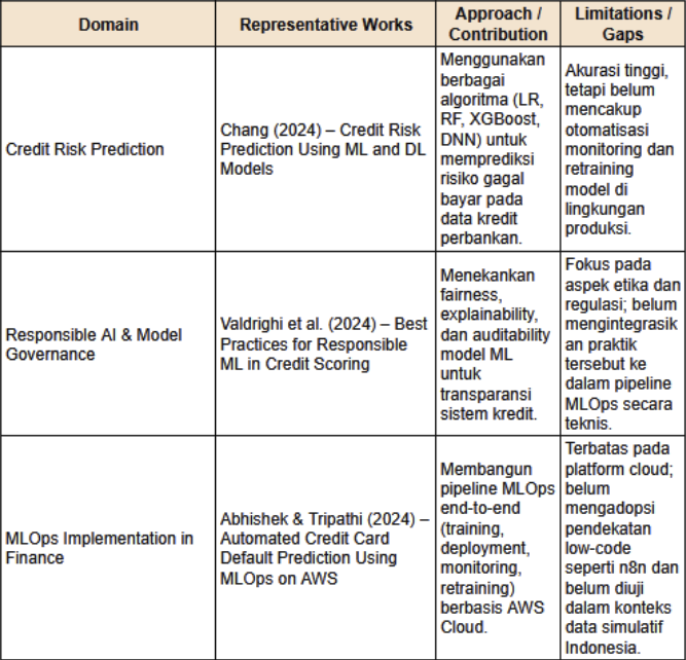
\includegraphics[width=0.8\textwidth]{bab2/Research_gap.png}
    \caption{\textit{Research gap} dari penelitian terdahulu}
    \label{fig:Research gap}
\end{figure}
\subsection*{1. Dasar Pemilihan Model \textit{Machine Learning}}
\textbf{Credit Risk Prediction Using Machine Learning and Deep Learning Models}
Penelitian tersebut mengkaji penerapan berbagai algoritma \textit{Machine Learning}, seperti Logistic Regression, Random Forest, XGBoost, dan Deep Neural Network, untuk memprediksi risiko gagal bayar pada data kredit perbankan. Hasil penelitian menunjukkan bahwa model berbasis \textit{ensemble learning} seperti XGBoost memiliki performa yang stabil dalam mendeteksi potensi gagal bayar nasabah. Temuan ini menjadi dasar pemilihan algoritma \textit{Machine Learning} yang digunakan dalam sistem analisis risiko kredit pada penelitian ini.\cite{sharma2021default}

\textbf{Credit Scoring Using Machine Learning and Deep Learning Techniques}
Penelitian ini merupakan studi komparatif terhadap beberapa algoritma pembelajaran mesin (SVM, LDA, DNN) untuk proses \textit{credit scoring}. Studi tersebut menekankan pentingnya pemrosesan data awal, seperti normalisasi dan penanganan ketidakseimbangan kelas (\textit{class imbalance}) pada \textit{dataset} kredit. Relevansinya adalah bahwa performa model yang dikelola dalam \textit{pipeline} MLOps sangat bergantung pada langkah pra-pemrosesan data (\textit{data preprocessing}) dan pemilihan model yang tepat.\cite{creditscoringml2024}

\subsection*{2. Justifikasi Kebutuhan \textit{Machine Learning Operations} (MLOps)}
\textbf{Automated Credit Card Default Prediction Using MLOps on AWS}
Penelitian memperkenalkan implementasi MLOps untuk prediksi gagal bayar kartu kredit menggunakan layanan AWS. \textit{Pipeline} yang dikembangkan mencakup tahapan \textit{model training, deployment, monitoring}, hingga \textbf{retraining otomatis} dengan integrasi CI/CD. Penelitian ini membuktikan bahwa penerapan MLOps dapat \textbf{mempercepat proses \textit{deployment} model hingga tiga kali lipat} dan menurunkan waktu \textit{downtime} model sebesar 40\%. Hasil ini memperkuat dasar bahwa integrasi MLOps sangat efektif dan diperlukan untuk menjaga performa model analisis risiko kredit di lingkungan produksi.\cite{creditscoringml2024}

\textbf{MLOps: Continuous Delivery and Automation Pipelines in Machine Learning}
Laporan teknis ini menjelaskan arsitektur dan praktik terbaik dalam implementasi MLOps, mencakup \textit{continuous integration}, \textit{continuous delivery}, \textit{model registry}, \textit{monitoring}, dan \textit{automated retraining}. Penelitian ini relevan karena memberikan gambaran arsitektur MLOps yang bersifat umum. Arsitektur tersebut kemudian diadaptasi dalam penelitian ini menggunakan \textit{low-code tool} n8n untuk mengatur \textit{pipeline} analisis risiko kredit otomatis berbasis data simulatif.\cite{Kreuzberger2023}

\subsection*{3. Aspek Regulasi dan Tata Kelola Model}
\textbf{Best Practices for Responsible Machine Learning in Credit Scoring}
Studi ini mengusulkan panduan penerapan \textit{Responsible AI} dalam konteks \textit{credit scoring} yang menyoroti aspek \textit{fairness}, \textit{explainability}, dan \textit{auditability} model. Penelitian ini menekankan bahwa sistem berbasis ML di sektor keuangan harus memiliki \textit{audit trail} dan dokumentasi yang jelas untuk memastikan transparansi keputusan kredit. Temuan ini menjadi rujukan penting dalam pengembangan \textit{pipeline} MLOps yang menjamin tata kelola (\textit{governance}) dan kepatuhan terhadap regulasi OJK dan Bank Indonesia.\cite{Valdrighi2024}

\subsection*{4. Pentingnya Pra-pemrosesan Data}
Berbagai studi komparatif mengenai \textit{credit scoring} menunjukkan bahwa performa prediktif model ML sangat bergantung pada kualitas data awal, terlepas dari kompleksitas algoritmanya. Langkah pra-pemrosesan yang andal penting, terutama dalam menangani ketidakseimbangan kelas (\textit{class imbalance}). Pada \textit{dataset} kredit, kasus gagal bayar (\textit{default}) umumnya merupakan kelas minoritas sehingga teknik penyeimbangan khusus diperlukan. Teknik seperti \textit{Synthetic Minority Over-sampling Technique} (SMOTE) membantu model ML mendeteksi pola \textit{default} secara lebih efektif. Keandalan langkah pra-pemrosesan ini secara langsung memengaruhi stabilitas model yang akan dioperasionalkan dalam \textit{pipeline} MLOps.
MLOps memainkan peran krusial dalam domain keuangan yang sangat teregulasi. Sistem MLOps yang terstruktur memungkinkan otomatisasi proses kepatuhan (\textit{compliance}) dan tata kelola (\textit{governance}). MLOps menyediakan kerangka kerja untuk memublikasikan, memantau, dan melatih ulang model secara teratur dengan menerapkan prinsip CI/CD. Prinsip tersebut menjamin konsistensi, akuntabilitas, dan auditabilitas yang menjadi tuntutan utama regulator seperti Otoritas Jasa Keuangan (OJK) dan Bank Indonesia.\cite{AIMSPress2024}
\subsection*{5. Fungsi Tata Kelola Keuangan}
MLOps memainkan peran krusial dalam domain keuangan yang sangat teregulasi. Sistem MLOps yang terstruktur memungkinkan otomatisasi proses kepatuhan (\textit{compliance}) dan tata kelola (\textit{governance}). MLOps menyediakan kerangka kerja untuk memublikasikan, memantau, dan melatih ulang model secara teratur dengan menerapkan prinsip CI/CD. Prinsip tersebut menjamin konsistensi, akuntabilitas, dan auditabilitas yang menjadi tuntutan utama regulator seperti Otoritas Jasa Keuangan (OJK) dan Bank Indonesia.\cite{rafi2024explainable}

\subsection*{6. Analisis Kesenjangan Penelitian (Research Gap)}

Berdasarkan telaah terhadap penelitian-penelitian terdahulu, dapat diidentifikasi bahwa mayoritas studi mengenai analisis risiko kredit berbasis \textit{Machine Learning} berfokus pada peningkatan akurasi model prediksi, khususnya melalui penggunaan algoritma \textit{ensemble learning} seperti XGBoost, Random Forest, dan Deep Neural Network.\cite {Chang2024} Namun demikian, sebagian besar penelitian tersebut masih menitikberatkan pada tahap eksperimentasi model (\textit{offline modeling}) dan belum membahas secara komprehensif aspek operasionalisasi model di lingkungan produksi.

Selain itu, penelitian terkait \textit{Machine Learning Operations} (MLOps) umumnya mengadopsi arsitektur berbasis \textit{cloud-native} atau \textit{hyperscale platform} seperti AWS, Azure, atau Kubeflow, yang memerlukan sumber daya infrastruktur dan kompetensi teknis tingkat lanjut. Pendekatan tersebut relatif sulit diadopsi oleh organisasi berskala kecil hingga menengah, khususnya dalam konteks industri keuangan di Indonesia yang memiliki keterbatasan sumber daya teknis.\cite{GoogleCloud2024}

Kesenjangan penelitian lainnya terletak pada minimnya kajian yang mengeksplorasi penggunaan \textbf{platform low-code} sebagai orkestrator utama dalam pipeline MLOps. Penelitian yang secara spesifik mengintegrasikan proses \textit{training, deployment, monitoring}, dan \textit{automated retraining} menggunakan alat \textit{low-code} seperti \textbf{n8n} masih sangat terbatas.

Berdasarkan hal tersebut, penelitian ini bertujuan mengisi celah tersebut dengan merancang dan mengimplementasikan \textit{pipeline} MLOps berbasis \textit{low-code} untuk analisis risiko kredit. Pipeline ini mengintegrasikan model \textit{Machine Learning} (XGBoost), \textit{model registry}, \textit{containerization}, serta mekanisme \textit{monitoring} dan \textit{continuous training} secara otomatis. Pendekatan ini diharapkan menjadi solusi yang lebih praktis, efisien, dan mudah direplikasi dalam konteks operasional lembaga keuangan di Indonesia. \cite{Sundberg2023}


\section{Teori/Konsep Dasar}

\subsection{Pra-Pemrosesan Data Lanjutan dalam Credit Scoring}

Selain teknik normalisasi dan penyeimbangan kelas, pemodelan risiko kredit juga memerlukan pendekatan pra-pemrosesan yang berfokus pada stabilitas dan interpretabilitas fitur. Salah satu teknik yang banyak digunakan dalam industri perbankan adalah transformasi \textit{Weight of Evidence} (WoE) dan pengukuran \textit{Information Value} (IV).\cite{venkatsai2025validation}

Transformasi WoE dilakukan dengan mendiskretisasi variabel numerik ke dalam beberapa \textit{bin}, kemudian menghitung rasio logaritmik antara proporsi debitur baik (\textit{non-default}) dan debitur gagal bayar (\textit{default}) pada setiap bin. Pendekatan ini menghasilkan fitur yang lebih stabil dan mudah diinterpretasikan, bahkan ketika digunakan pada model \textit{black-box} seperti XGBoost.\cite{ye2025unlocking}

Sementara itu, \textit{Information Value} (IV) digunakan sebagai metrik seleksi fitur untuk mengukur kekuatan prediktif suatu variabel terhadap risiko gagal bayar. Variabel dengan nilai IV yang sangat rendah dianggap tidak informatif, sedangkan nilai IV yang terlalu tinggi dapat mengindikasikan potensi \textit{data leakage}.\cite{maurino2025data}

Penggunaan WoE dan IV memiliki relevansi langsung dengan implementasi MLOps, karena fitur yang lebih stabil mempermudah proses pemantauan \textit{data drift}. Dalam konteks ini, perubahan distribusi fitur WoE dapat dideteksi secara kuantitatif menggunakan metrik seperti \textit{Population Stability Index} (PSI), yang selanjutnya digunakan sebagai pemicu proses \textit{retraining} otomatis dalam pipeline MLOps.\cite{Chang2024}


\subsection{Analisis Risiko Kredit}
Analisis risiko kredit merupakan proses penilaian kemampuan calon nasabah dalam memenuhi kewajiban pembayaran pinjaman. Tujuan utama analisis risiko kredit adalah untuk meminimalkan kemungkinan terjadinya \textbf{gagal bayar (\textit{credit default})}. Secara tradisional, lembaga keuangan menggunakan pendekatan analisis 5C (\textit{Character, Capacity, Capital, Condition, Collateral}). Namun pendekatan ini sering kali bersifat subjektif dan kurang adaptif. Dengan kemajuan \textit{Machine Learning}, proses penilaian risiko kredit dapat dilakukan lebih otomatis dan akurat melalui analisis data historis dan pola transaksi. \cite{ojk2024pojk29}
\subsection{Kalkulasi Risiko Kredit}
Kalkulasi risiko kredit adalah proses kuantifikasi potensi kerugian finansial yang dapat dialami lembaga keuangan akibat gagal bayar debitur. Salah satu metrik utama dalam manajemen risiko kredit adalah \textit{Expected Loss} (EL), yang dihitung sebagai:

\[
\text{EL} = \text{PD} \times \text{LGD} \times \text{EAD} 
\]
\begin{itemize}
    \item \textbf{PD (\textit{Probability of Default})}: Probabilitas bahwa debitur akan gagal memenuhi kewajiban pembayaran dalam periode tertentu. Nilai ini merupakan target utama prediksi dari model \textit{Machine Learning}.
    \item \textbf{LGD (\textit{Loss Given Default})}: Persentase kerugian yang dialami bank jika debitur gagal bayar.
    \item \textbf{EAD (\textit{Exposure at Default})}: Total nilai pinjaman yang terekspos saat gagal bayar terjadi.
\end{itemize}
Dengan mengotomatisasi perhitungan PD dan memantau performa model yang menghasilkan nilai tersebut, penerapan MLOps dapat meningkatkan akurasi dan keandalan kalkulasi risiko kredit.\cite{Chang2024}

\subsection{\textit{Machine Learning} dalam Analisis Risiko Kredit}
\textit{Machine Learning} memungkinkan pembangunan model \textit{credit scoring} yang secara otomatis mengklasifikasikan calon debitur ke dalam kategori “layak” atau “berisiko”. Algoritma yang sering digunakan antara lain:
\begin{itemize}
    \item Logistic Regression
    \item Random Forest dan XGBoost
    \item Neural Network
\end{itemize}
Model \textit{ensemble} seperti XGBoost dapat meningkatkan akurasi prediksi.\cite{mlopsbanking2025}

\subsection{Credit Scoring dan Model Drift}
\textbf{\textit{Model drift}} adalah penurunan performa model akibat perubahan distribusi data. Dua jenis \textit{drift} utama yang relevan dalam \textit{credit scoring} adalah:
\begin{itemize}
    \item \textbf{\textit{Data drift}}: perubahan pada distribusi input (misalnya, perubahan demografi nasabah).
    \item \textbf{\textit{Concept drift}}: perubahan hubungan antara input dan target (misalnya, krisis ekonomi mengubah perilaku gagal bayar).
\end{itemize}
MLOps diperlukan untuk mengatasi masalah ini melalui mekanisme \textit{monitoring}, \textit{alerting}, dan \textit{retraining} model secara otomatis. \cite{nikolaidis2022credit}

\subsection{Evaluasi Kinerja Model dan Transformasi ke Keputusan Operasional}

Evaluasi kinerja model prediksi risiko kredit tidak hanya berfokus pada akurasi global, tetapi juga pada kemampuan model dalam membedakan debitur berisiko tinggi dan rendah. Oleh karena itu, metrik evaluasi yang umum digunakan meliputi \textit{Area Under the Curve} (AUC), \textit{F1-Score}, dan \textit{Kolmogorov-Smirnov (K-S) Statistic}.\cite{venkatsai2025validation}

Statistik K-S memiliki peran penting dalam konteks operasional, karena digunakan untuk menentukan ambang batas (\textit{cut-off}) skor kredit yang optimal. Ambang batas ini merepresentasikan titik pemisahan maksimum antara distribusi probabilitas debitur baik dan debitur gagal bayar, sehingga dapat diterjemahkan secara langsung menjadi kebijakan kredit.

Output model berupa nilai \textit{Probability of Default} (PD) selanjutnya ditransformasikan ke dalam bentuk \textit{credit scorecard} dan \textit{risk grade} institusional. Proses ini memungkinkan hasil prediksi model untuk diintegrasikan secara otomatis ke dalam sistem pengambilan keputusan kredit, seperti keputusan \textit{approve}, \textit{reject}, atau \textit{manual review}, yang diorkestrasi melalui pipeline MLOps.\cite{nikolaidis2022credit,mlopsdrift2025}


\subsection{Konsep \textit{Machine Learning Operations} (MLOps)}
MLOps merupakan integrasi DevOps dengan siklus hidup \textit{Machine Learning} (\textit{training}, \textit{deployment}, \textit{monitoring}, \textit{retraining}). Komponen utama MLOps meliputi:
\begin{itemize}
    \item Data Pipeline
    \item Model Pipeline
    \item Deployment Pipeline
    \item Monitoring \& Retraining
\end{itemize}
\textbf{CI (\textit{Continuous Integration})}, \textbf{CD (\textit{Continuous Delivery})}, dan \textbf{CT (\textit{Continuous Training})} adalah fondasi utama dari MLOps.\cite{Nogare2023}

\subsection{Explainable AI (XAI) dan Kepatuhan Regulasi}

Dalam sektor keuangan yang sangat teregulasi, model \textit{Machine Learning} tidak hanya dituntut memiliki performa tinggi, tetapi juga harus dapat dijelaskan (\textit{explainable}) dan dapat diaudit. Regulasi menuntut lembaga keuangan untuk mampu memberikan alasan yang jelas atas setiap keputusan kredit, khususnya pada kasus penolakan pinjaman.

Model \textit{ensemble learning} seperti XGBoost bersifat \textit{black-box} moderat, sehingga memerlukan metode penjelasan pasca-pelatihan (\textit{post-hoc explanation}). Salah satu pendekatan yang paling banyak digunakan adalah \textit{SHapley Additive exPlanations} (SHAP), yang mampu memberikan penjelasan baik secara lokal (tingkat individu) maupun global (tingkat model).\cite{yotsawat2021improved}

Integrasi XAI ke dalam pipeline MLOps memungkinkan setiap prediksi kredit tidak hanya menghasilkan nilai PD, tetapi juga disertai dengan penjelasan kontribusi fitur. Informasi ini dicatat sebagai bagian dari \textit{audit trail}, sehingga mendukung aspek transparansi, akuntabilitas, dan kepatuhan regulasi terhadap ketentuan Otoritas Jasa Keuangan (OJK) dan Bank Indonesia.\cite{ye2025unlocking}

\subsection{Low-Code Workflow Automation (n8n)}
n8n adalah \textit{tool} \textit{low-code} yang digunakan untuk mengotomatisasi \textit{workflow} secara visual. Dengan n8n, \textit{pipeline} MLOps dapat dibangun tanpa \textit{scripting} yang kompleks. Pendekatan ini mencakup tahapan \textit{data preparation, training, deployment,} dan \textit{alerting}. Pendekatan \textit{low-code} ini cocok untuk organisasi kecil-menengah dan relevan dengan penelitian ini yang bertujuan merancang \textit{pipeline} MLOps yang efisien.\cite{Sundberg2023}



